\begin{comment}
\chapter{Diseño}
\section{Diseño de boya para nodos sensores y nodo concentrador}
\section{Diagrama de circuito fuente de alimentacion}
\section{Diagrama de circuitos de nodo sensor}
\section{Diagrama de circuitos de nodo concentrado}
\section{Diseño de boya para nodo sensor}
\section{Diagrama de comunicacion del nodo concentrador con el servidor}
\section{Diseño de Base de datos}
\section{Modelo Relacional}
\section{Arquitectura}
\section{Diagramas UML}
\section{Diagramas de caso de uso}
\section{Diagramas de secuencia}
\section{Diccionario de Datos}
\section{Diseño de Mock-up para la pagina web}
\section{Pagina principal}
\section{Diseño de la interfaz para la página Web}
\section{Integracion Final del Sistema}
\section{Escenario de pruebas}    
\end{comment}

%opcion 2

\chapter{Diseño}

\section{Diseño del Sistema}
\subsection{Arquitectura del Sistema}
\subsection{Diseño de boya para nodos sensores y nodo concentrador}

\section{Diseño de Hardware}

\subsection{Diagrama eléctrico de los nodos}
\label{sec:diagrama_electrico}

La red está conformada por nodos sensores y un nodo concentrador. Cada nodo sensor se encarga de medir parámetros físico-químicos del agua y transmitir la información recopilada hacia el nodo final, el cual actúa como concentrador. Con base en los componentes analizados y seleccionados en capítulos anteriores, se presenta el diseño esquemático del circuito electrónico del nodo sensor (Figura~\ref{fig:esquema_nodo_sensor}).

\subsection*{Descripción general del circuito}

El circuito del nodo sensor se compone de dos microcontroladores principales: un \textbf{PIC16F1823} y un \textbf{Xiao ESP32-S3}. El primero se encarga del sensado y control energético, mientras que el segundo maneja la comunicación inalámbrica con el siguiente nodo (o concentrador) a través de un módulo \textbf{Wi-Fi HaLow FGH100M}.

\begin{itemize}
    \item \textbf{PIC16F1823}: gestiona la activación secuencial de los sensores mediante un demultiplexor \textbf{74HC238}, activando solo un sensor a la vez para minimizar el consumo energético. Los sensores analógicos (pH, conductividad, OD, turbidez) son activados por MOSFETs \textbf{AO3400A} y su señal de salida se dirige a entradas ADC del PIC.
    
    \item \textbf{Sensor de temperatura DS18B20}: se conecta directamente al PIC mediante una línea digital dedicada para adquisición por protocolo 1-Wire.

    \item \textbf{Demultiplexor 74HC238}: permite seleccionar cuál de los sensores analógicos se activa en cada momento, controlado por tres líneas digitales del PIC.

    \item \textbf{Xiao ESP32-S3}: se encarga de la comunicación inalámbrica. Recibe los datos procesados por el PIC a través de un canal \textbf{UART}, y los transmite al siguiente nodo o al concentrador mediante el módulo HaLow conectado en sus pines digitales.

    \item \textbf{Módulo HaLow FGH100M}: es operado por el Xiao ESP32 y sirve como interfaz de comunicación bajo el estándar IEEE 802.11ah.

    \item \textbf{Fuente de alimentación}: el sistema se alimenta desde una batería Li-ion de 3.7 V regulada por un cargador solar \textbf{CN3065}. La salida alimenta un convertidor \textbf{step-up} que genera 5V, y un LDO que provee 3.3V para los componentes lógicos.
\end{itemize}

\begin{figure}[H]
\centering
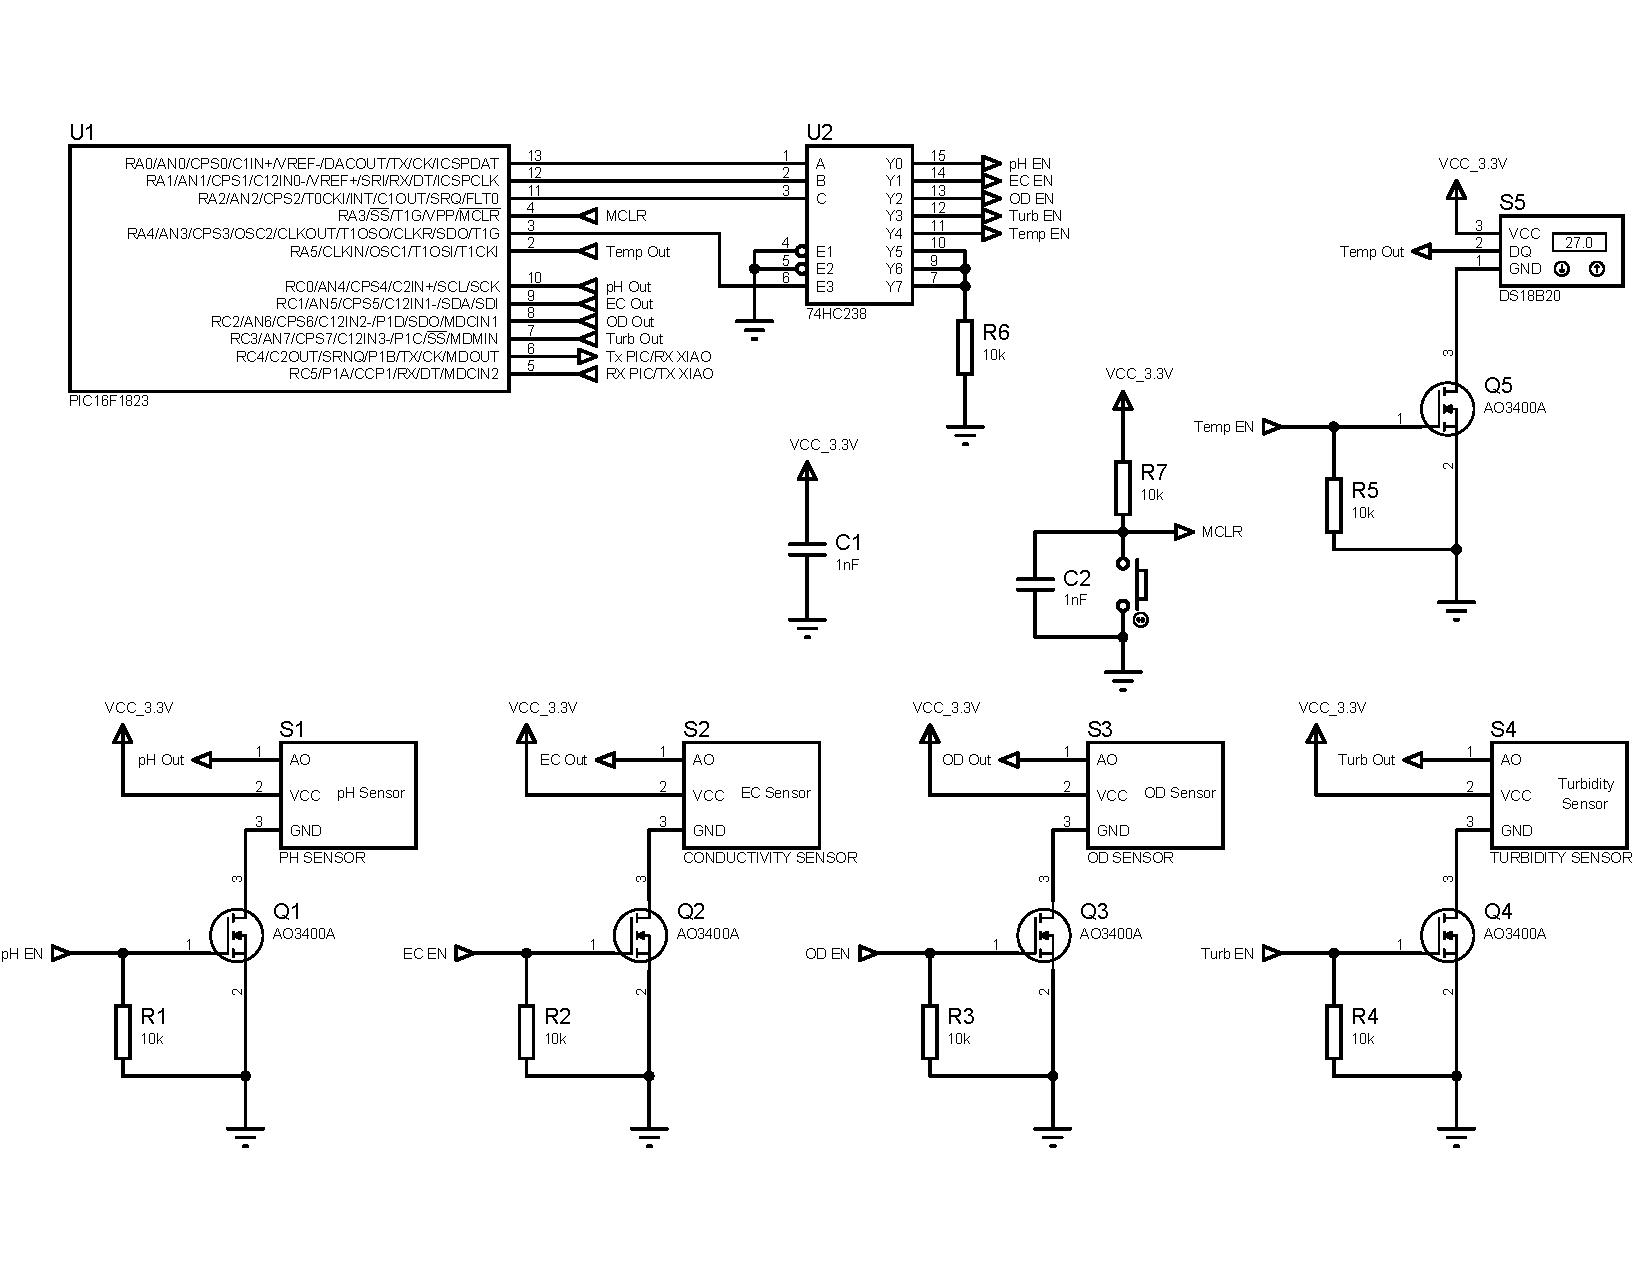
\includegraphics[width=0.8\textwidth]{Documento/Imagenes/Diseño/Diagramas electricos/Controller Sensor_fit.pdf}
\caption{Diagrama eléctrico del control de sensores.}
\label{fig:esquema_nodo_sensor}
\end{figure}

\begin{figure}[H]
\centering
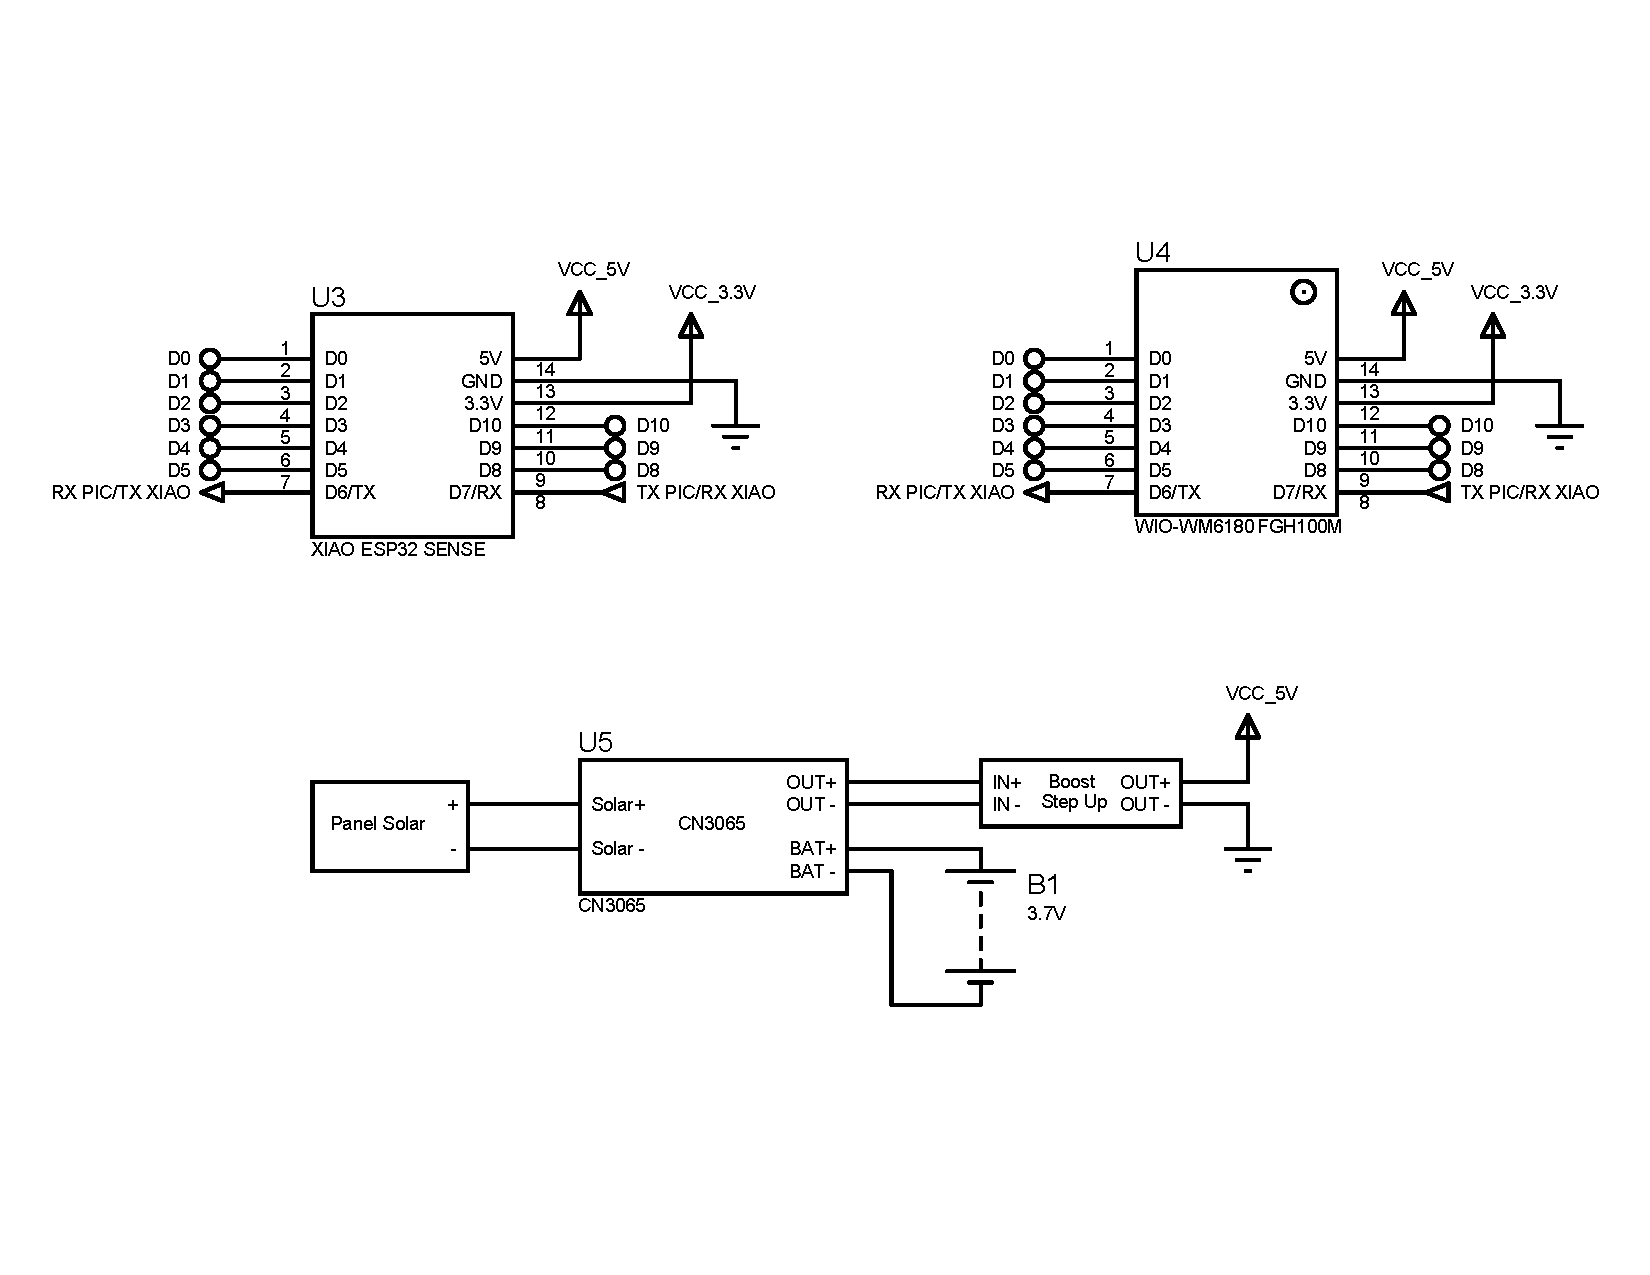
\includegraphics[width=0.8\textwidth]{Documento/Imagenes/Diseño/Diagramas electricos/microcontroller_fit.pdf}
\caption{Diagrama eléctrico comunicación inalámbrica y fuente de alimentación.}
\label{fig:esquema_nodo_sensor2}
\end{figure}


\subsection*{Funcionamiento del sistema}

Durante cada ciclo de adquisición:

\begin{enumerate}
    \item El PIC activa uno por uno los sensores mediante el demultiplexor y sus respectivas compuertas MOSFET.
    \item Cada sensor permanece encendido aproximadamente 5 segundos para estabilizar la medición.
    \item El PIC adquiere los valores analógicos o digitales, almacena las lecturas y las envía por UART al Xiao ESP32.
    \item El Xiao ESP32 activa la cámara, captura una imagen (JPG), y empaqueta los datos sensados junto con la imagen.
    \item Finalmente, activa el módulo HaLow para transmitir toda la información al nodo siguiente o al nodo concentrador.
    \item Al finalizar, el sistema entra en modo \textit{sleep} hasta el próximo ciclo.
\end{enumerate}



\section{Diseño de Software}
\begin{table}[H]
\centering
\caption{Tabla Nodo.}
\label{tab:usuario}
\begin{tabular}{|l|l|l|}
\hline
\textbf{Campo}              & \textbf{Tipo de dato} & \textbf{Llave}   \\ \hline
idNodo                  & int                   & primaria         \\ \hline
Nombre                    & varchar               & N/A              \\ \hline
apellido                  & varchar               & N/A              \\ \hline
seg\_apellido             & varchar               & N/A              \\ \hline
correo                    & varchar               & N/A              \\ \hline
fecha\_nacimiento         & date                  & N/A              \\ \hline
genero                    & varchar               & N/A              \\ \hline
bandera\_administrador    & tinyint               & N/A              \\ \hline
nodo                      & int                   & N/A              \\ \hline
\end{tabular}
\end{table}

\subsection{Conexión entre nodos, concentrador y servidor}.

En el sistema propuesto, los nodos sensores distribuidos a lo largo del entorno fluvial establecen comunicación con un nodo concentrador central mediante una red inalámbrica local basada en el estándar Wi-Fi HaLow (IEEE 802.11ah). Esta tecnología opera en la banda sub-1 GHz, lo cual le otorga ventajas significativas en términos de alcance (hasta 1 km en condiciones ideales) y penetración en entornos con vegetación densa, además de un consumo energético moderado que favorece la operación autónoma con baterías o paneles solares.

El nodo concentrador cumple una función crítica dentro de la arquitectura, ya que actúa como gateway inalámbrico. Es decir, se encarga de recibir la información sensorial proveniente de los nodos HaLow y reenviarla al servidor central utilizando una interfaz de red externa. Esta interfaz puede implementarse mediante un módulo de red celular (4G/5G), ideal para zonas con baja infraestructura de conectividad, o a través de una red WLAN convencional (2.4/5 GHz) disponible en estaciones fijas cercanas al sitio de monitoreo.

Para establecer la comunicación entre el nodo concentrador y el servidor, se asume que el concentrador cuenta con dicha interfaz de red externa, permitiendo el envío de datos a través del protocolo HTTP. Esta suposición garantiza la interoperabilidad con servicios web modernos y facilita la integración con plataformas de almacenamiento, análisis o visualización de datos.

Una vez recibidos, los datos son procesados por el servidor y almacenados en una base de datos estructurada, permitiendo su consulta posterior, análisis automatizado o incluso la generación de comandos que puedan enviarse de regreso a los nodos sensores, habilitando así una comunicación bidireccional dentro del sistema.


\subsection{Base de datos}
\subsubsection{Diseño de base de datos}
\subsubsection{Modelo Relacional}
\subsubsection{Diccionario de datos}

\section{Diseño de Comunicación}
\subsection{Diagrama de comunicación del nodo concentrador con el servidor}

\section{Diseño de Interfaces de Usuario}
\subsection{Diseño de Mock-up para la página web}
\subsection{Página principal}

\section{Modelado del Sistema}
\subsection{Diagramas UML}
\subsubsection{Diagramas de caso de uso}
\subsubsection{Diagramas de secuencia}

\section{Integración y Pruebas}
\subsection{Integración final del sistema}
\subsection{Escenario de pruebas}
